% !TeX spellcheck = en_US
\documentclass[./main.tex]{subfiles}
\begin{document}

\section{Relevant links}

\begin{itemize}
	\item \href{https://github.com/commed-it/backend}{GitHub backend repository}
	\item \href{https://github.com/commed-it/mobile-app}{GitHub Mobile App repository}
	\item \href{https://github.com/commed-it/web-client}{GitHub Web client repository}
	\item \href{https://github.com/commed-it/docs}{GitHub docs}
	\item \href{https://github.com/orgs/commed-it/projects/1}{GitHub project management}
	\item \href{https://drive.google.com/drive/folders/15iM-Fm6krEBcHkVyaqSUfjJMY1MKBMm6?usp=sharing}{Slides of the presentation}
	\item \href{https://docs.google.com/spreadsheets/d/1qyKpYXf7lZ2p7q09JHzv7e7yGVBiPEqGNHhwPsFYcXc/edit?usp=sharing}{Spreadsheet documentation}
\end{itemize}

\section{Planification}

\subsection{User Stories}

The first thing that was done regarding the planification of the project
was to define the behavior of the application in a list of user stories.
The next list exposes all of the actions that the user can do with it as
well as different ways of interacting with it. It has to be noted that for this Sprint 
there has been no changes on the user stories.

\begin{itemize}
	\item \textbf{AUTH1}: As a guest, I want to register in the application 
	\item \textbf{AUTH2}: As a user, I want to log in to the application. 
	\item \textbf{AUTH3}: As a registered user, I want to create a profile of my company.
	\item \textbf{PROD1}: As a guest, I want to search for services or products so that I receive a list of services or products.
	\item \textbf{PROD2}: As a guest, I want to have a detailed view of the product/service.
	\item \textbf{PROD3}: As a registered user who has a company profile, I want to create services/products.
	\item \textbf{CHAT1}: As a user, I want to connect to a company because of a publication.
	\item \textbf{CHAT2}: As a user, I need to chat with the company that I connected with.
	\item \textbf{CHAT3}: As a company, I want to chat with the users that have sent a message.
	\item \textbf{FO1}: As a company, I want to send the Formal Offer which contains the contract pdf through the chat.
	\item \textbf{FO2}: As a company, I want to digitally sign contracts.
	\item \textbf{FO3}: As a user, I want to digitally sign contracts.
	\item \textbf{FO4}. As a company, I want to have a list of my sent formal offers.
	\item \textbf{FIN1}: As Commed, I want to get a 5\% commission on each contract.
	\item \textbf{FIN2}: As a company, I want to publish the first 3 announcements freely.
	\item \textbf{FIN3}: As a company, I want to have the possibility to pay to promote my announcements.
\end{itemize}
\subsection{Scrum organization and planification}
Afterwards, a meeting was held in order to fulfill the product backlog
with all the tasks that had to be done. These tasks were related to User
Stories, but they were divided so that the product backlog had a small
granularity in the given tasks. Some tasks were leftovers from the second sprint, as 
it was intended to have the integration with the API done by the end of it, but 
the team didn't have enough time to implement them.
\\
\\
According to the kanban, it has been created a milestone named \textit{Sprint  3}, which groups all the issues from this Sprint. It has also been migrated the leftovers from the \textit{Sprint 2} to the new milestone.
% TODO change figure
\begin{figure}[H]
	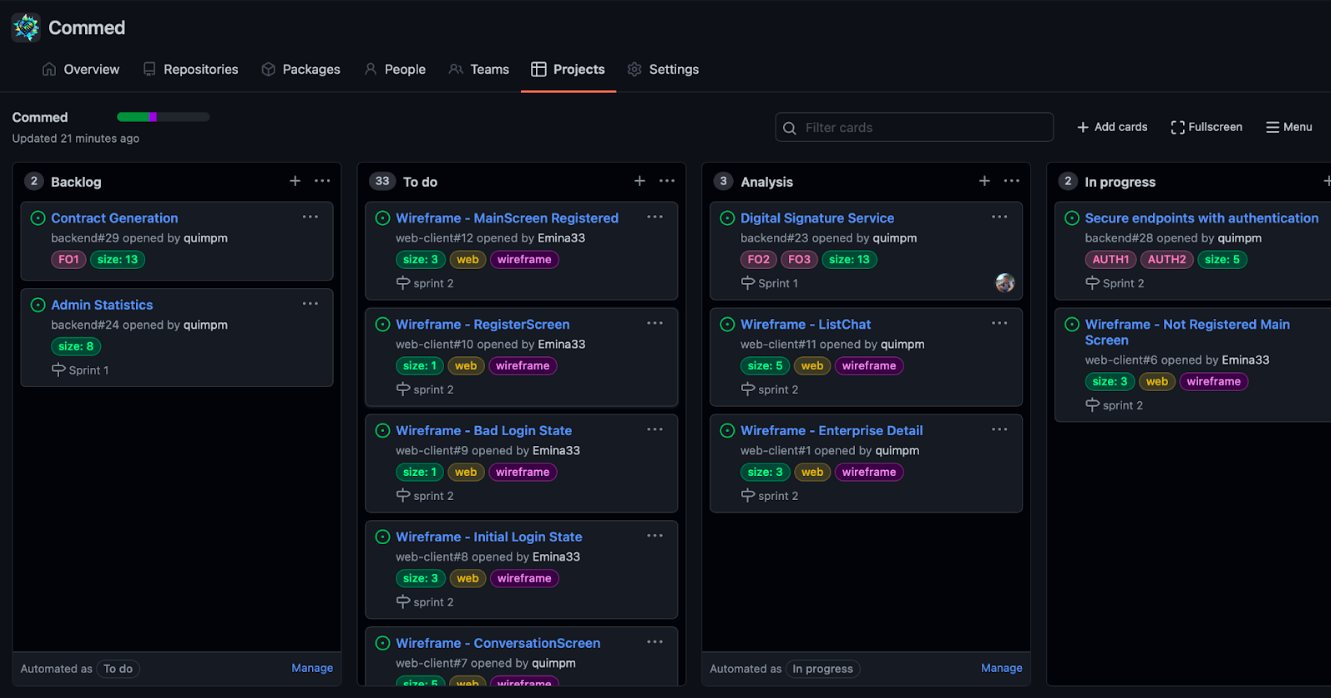
\includegraphics[width=15cm]{img/kanban.png}
	\caption{Screenshot of the last days of the project kanban.}
\end{figure}
\subsubsection{Issues}
\textbf{Backend}
\begin{verbatim}
- Upgrade Docker
	- size: 1
- Chat Feature Implementation
	- size : 13
- Fix Product Images CRUD
	- size: 13
- FormalOffer in Admin
	- size: 1
- Enterprise Profile Image and Banner
	- size: 1
- Fix List Formal Offers
	- size: 2
- Fix List chat encounters
	- size: 2
- Add Endpoint for starting chat
	- size: 3
- Add better mocks
	- size: 3
\end{verbatim}
\textbf{Web client}
\begin{verbatim}
- Sending FormalOffer frm Chat
    - size: 5
- Implementation of Formal Offer Form
    - size: 5
- Implementation of Chat
    - size: 8
- WebClient NavBar fixes
    - size: 3
- WebClient Labels
    - size: 2
- Recommendations algorithm Location
    - size: 2
\end{verbatim}
\textbf{Mobile application}
\begin{verbatim}
- Implementation of Authentication with the API
    - size: 8
- Implementation of FormalOffer API backend Integration with flutter
    - size: 5
- Implementation of Chat API Integration
    - size: 13
- Implementation of Search feature with the API in mobile
    - size: 8
- Implementation of Product/Service/Publication integration
    - size: 5
- Implement application labels
    - size: 1
- Application NavBar fixes
    - size: 3
\end{verbatim}

\subsection{Scrum analytics}
As Github does not support milestones for a group of repositories but for single one, it has been created three different milestones for each project: \texttt{backend}, \texttt{web-client} and \texttt{mobile-app}.
\\
\\
\textbf{backend}
\begin{figure}[H]
	\centering
	
\includegraphics[width=15cm]{img/sprint3-backend.png}
	\caption{Backend Sprint 3 milestone}
\end{figure}
As it can be seen, the backend has only a few issues but some big ones. The implementation of Chat was one of the biggest use cases that was implemented, and integrating it with the web client and the mobile application was not an easy task. Also, it was thought at first that solving a bug regarding the product images would be an easy task, but it took as much as the chat implementation itself, as a lot of tasks regarding the analysis was needed before being able to implement a correct way.
\\
\\
\textbf{web-client}
\begin{figure}[H]
	\centering
	
\includegraphics[width=15cm]{img/sprint3-web.png}
	\caption{Web client Sprint 3 milestone}
\end{figure}
Regarding the web client, all of the tasks assigned for this Sprint are done.  The main topic in the web client was polishing things and making the chat work, as well as the formal offers.
\\\\
\textbf{mobile-app}
\begin{figure}[H]
	\centering
	
\includegraphics[width=15cm]{img/sprint3-mobile.png}
	\caption{Web client Sprint 3 milestone}
\end{figure}
In this sprint, the API integration was  done in he mobile application. It was also polished some things for the user experience.
%Sprint stuff. Commits estatistics, completition of the tasks, number of tasks done, amount of size completed, sprint progression grapic, Backlog...

\section{Requirements}
In this section the list of requirements that the application has to offer to the user are on the list below. As matter of fact, the requirements were left as they were in the previous Sprint, as no new ones or refinements were found. 
\\\\
\textbf{Functional Requirements:}
\begin{itemize}
	
	\item
	The application has to let all kinds of users search for products or
	services.
	\item
	The application has to let users register into the application and it will create automatically an enterprise profile.
	\item
	The application has to let users log in to the application if they
	have an active account on the system.
	\item
	The application has to let logged users publish products or services in the web application.
	\item
	The application has to let logged users interested in either a product
	or a service to start a chat with the owner of it.
	\item
	The application has to let logged users who are owners of a given
	product to chat with said interested users through a chat.
	\item
	The application has to let logged users send a commercial transaction
	contract when an agreement has been reached .
	\item 
	The application has to let logged users download a commercial transaction
	contract sent by the owner of a product that they are interested.
	\item
	The application has to let logged users sign a commercial transaction
	contract sent by the owner of a product that they are interested.
	\item
	The application has to generate the evidences for both sides of the
	commercial agreement.
	\item The application has to let logged users to view a list of the formal offers they are in.
\end{itemize}
\textbf{Non-Functional Requirements:}
\begin{itemize}
	
	\item
	The application has to be the most usable possible.
	\item
	The application has to be compliant and respect the laws that run in
	each country that it's available in.
	\item
	The application mustn't have large waiting times for the client.
	\item
	The application has to be portable and easy to deploy.
	\item
	The application has to be scalable and always leave the code open to
	the possibility of adding new features in the future.
\end{itemize}


\section{Main use cases}

\begin{figure}[H]
\centering
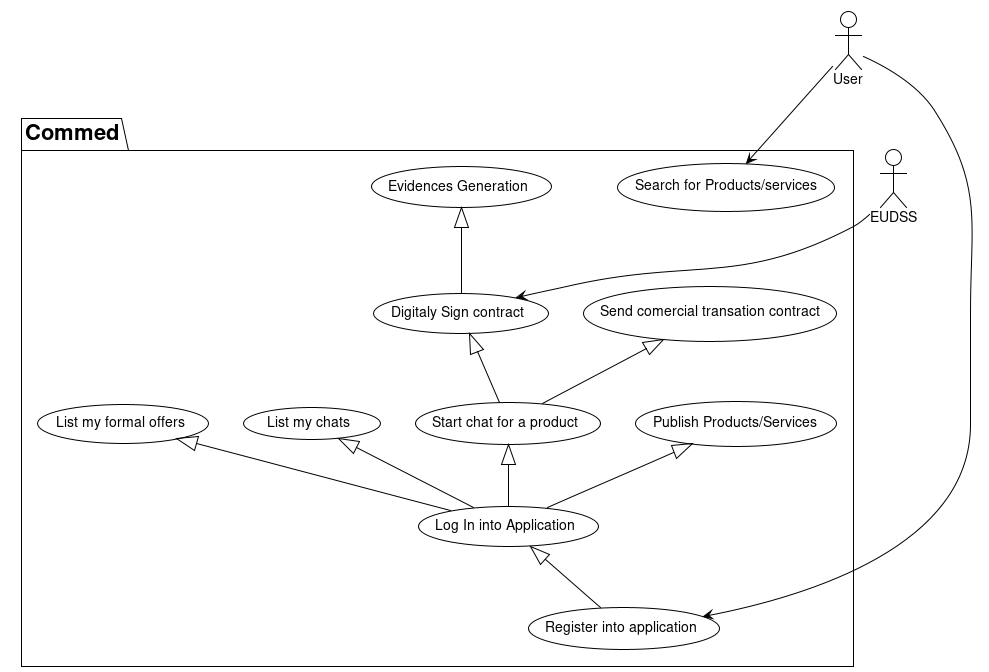
\includegraphics[width=\linewidth]{use_case_diagram/usecase_diagram.png} %TODO Update with new Use Cases file at ./use_case_diagram
\caption{Use case diagram of the application.}
\end{figure}

The use cases will be described as:

\begin{itemize}

\item
  \textbf{Register into application}

  \begin{itemize}
  
  \item
    \textbf{Actors:} User
  \item
    \textbf{Purpose:} Let a user register into the application system
  \item
    \textbf{Description:} Provides a screen with a form in which the
    user is able to fulfill it and send the information to the system in
    order to be registered.
  \end{itemize}
\item
  \textbf{Log In into Application}

  \begin{itemize}
  
  \item
    \textbf{Actors:} User
  \item
    \textbf{Purpose:} Log in to the application to be able to use some
    of the application services.
  \item
    \textbf{Description:} Provides a screen with a form in which the
    user will put its email and password. Then, they will log into the
    application so that they can start using the services that it provides.
  \end{itemize}
\item
  \textbf{Search for Products/services}

  \begin{itemize}
  
  \item
    \textbf{Actors:} User
  \item
    \textbf{Purpose:} Search for any product or service the user is
    interested in.
  \item
    \textbf{Description:} Provides a searcher for every user so that
    they can look up the products or services that they are interested
    in.
  \end{itemize}
\item
  \textbf{Publish Products/Services}

  \begin{itemize}
  
  \item
    \textbf{Actors:} User
  \item
    \textbf{Purpose:} Publish services or products in order to be sold
    to other users.
  \item
    \textbf{Description:} Lets a logged user publish the products and
    services that they offer in order for them to be sold to other
    interested users.
  \end{itemize}
\item
  \textbf{Start chat for a product}

  \begin{itemize}
  
  \item
    \textbf{Actors:} User
  \item
    \textbf{Purpose:} Users can start a chat when they are interested in
    a product
  \item
    \textbf{Description:} Lets a logged user start a chat with the
    owners of either a product or a service that they are interested in,
    so that they can start a negotiation.
  \end{itemize}
\item
  \textbf{Send commercial transaction contract}

  \begin{itemize}
  
  \item
    \textbf{Actors:} User
  \item
    \textbf{Purpose:} Send a formal offer with a commercial transaction
    contract.
  \item
    \textbf{Description:} Lets the owners of given products or services
    send a formal offer containing a compliant commercial transaction
    contract within the chat in which the negotiations are taking place.
  \end{itemize}
\item
  \textbf{Digitally Sign contract}

  \begin{itemize}
  
  \item
    \textbf{Actors:} User EUSSD
  \item
    \textbf{Purpose:} Sign a commercial transaction contract sent within
    a Formal Offer.
  \item
    \textbf{Description:} Lets the users of the application sign
    digitally the contract that was sent as a Formal Offer in the chat
    in which the negotiations took place.
  \end{itemize}
\item
  \textbf{Evidences Generation}

  \begin{itemize}
  
  \item
    \textbf{Actors:} User
  \item
    \textbf{Purpose:} Provide users with evidences and the billing of a
    business transaction
  \item
    \textbf{Description:} The system will generate for both parts the
    commercial transaction with all the evidences and the billing of
    the contract.
  \end{itemize}
\item
\textbf{List my chats}

\begin{itemize}
	
	\item
	\textbf{Actors:} User
	\item
	\textbf{Purpose:} Provides the user a list of the current opened chats with other users.
	\item
	\textbf{Description:} The system will query the current chats for a user, either if they are the product owner or the client.
\end{itemize}

\item
\textbf{List my formal offers}

\begin{itemize}
	
	\item
	\textbf{Actors:} User
	\item
	\textbf{Purpose:} Provides the user a list of the current formal offers with other users.
	\item
	\textbf{Description:} The system will query the current formal offers for a user, either if they are the product owner or the client.
\end{itemize}
\end{itemize}

\hypertarget{general-architecture}{%
\section{General architecture}\label{general-architecture}}

\begin{figure}[H]
\centering
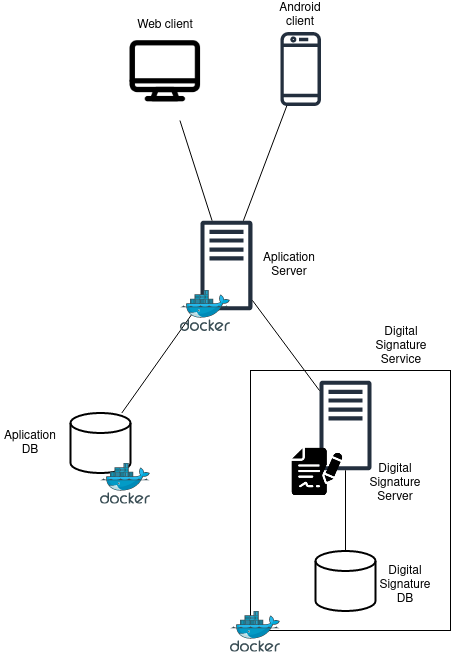
\includegraphics[width=0.6\textwidth]{architecture_diagram/Architecture.drawio.png}
\caption{General architecture of the application.}
\end{figure}

\subfile{backend.tex}

\subfile{mobile.tex} % TODO Add in these files
\subfile{frontend.tex} % TODO Add in these files - Done to review

\section{Database model}
The database model can be seen at figure \ref{fig:model-uml}.
% TODO Sergi Change database to add messages and other kinds of stuff
\begin{figure}[H]
\centering
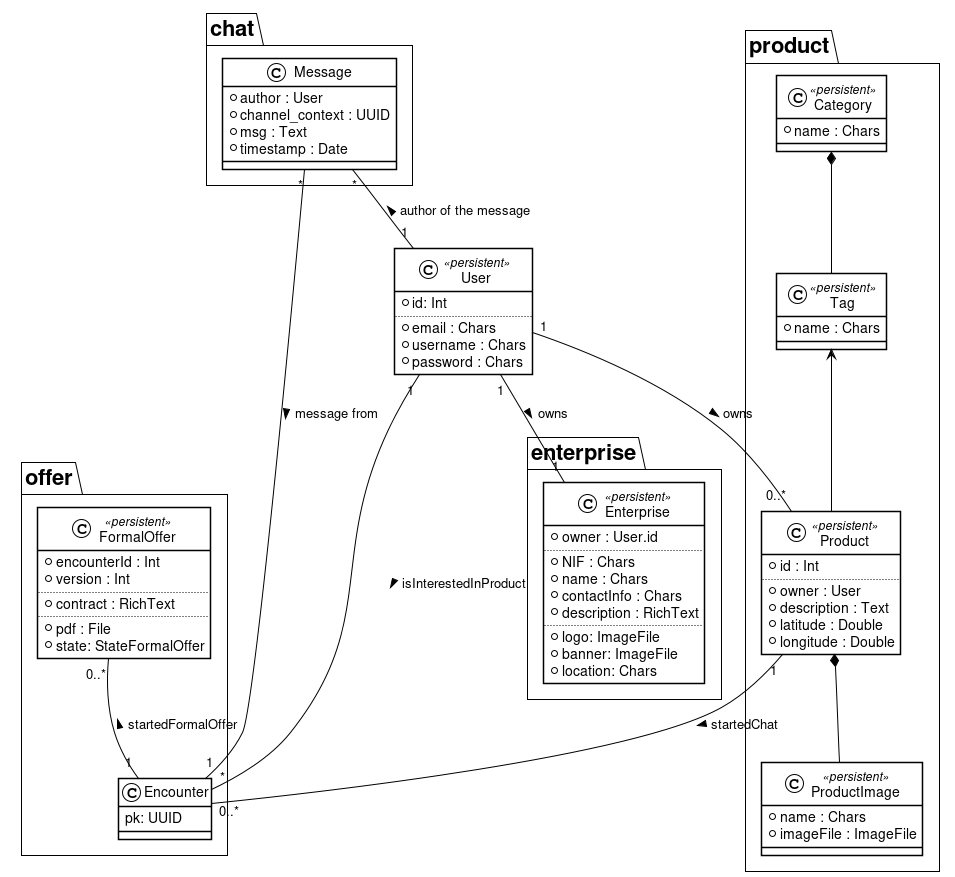
\includegraphics[width=\linewidth]{img/database-model-new.png}
\caption{UML diagram of the models.}
\label{fig:model-uml}
\end{figure}

\subsection{Modifications on the models}
The logo and the banner for an \texttt{Enterprise} had been finally added to the enterprise model, as well as  location of it. It has also been changed the \texttt{FormalOffer} model, changing the name of \texttt{signedPDF} to \texttt{PDF}, and allowing nulls on it, as some formal offers won't have any documents. It was added a field for storing the state of the formal offer, and although now it has only two states possible, some detected use cases have more than the naive thought that a document can either be signed on unsigned. It has been made it an immutable model, that is, it can only create instances and it cannot modify any of them, as it was thought that adding in the version of the document with another state was better than updating the database. This lets the chat mesmerize the state of a formal offer, so it doesn't modify it overtime if they patch the formal offer.\\
\\
Finally, it has been added a Message model, that holds the information on the messages, and having fields regarding the author, the time of creation, the author and the message itself. This last field stores a JSON with the values that were sent on it, as it will only be needed in a JSON format and won't be queried against its parameters. Moreover, it simplifies the querying of a normalized database, as it holds different types of messages, which for now it's only \texttt{FormalOffer}s and text messages.
\section{Main Screens} \label{sec:views}
%TODO delete it, maybe?
In the first stage of the designing of the mobile application, it was held a state diagram to start representing the management and the navigation of the user. This diagram can be shown in \ref{fig:stateapp}.
\begin{figure}[H]
	\centering
	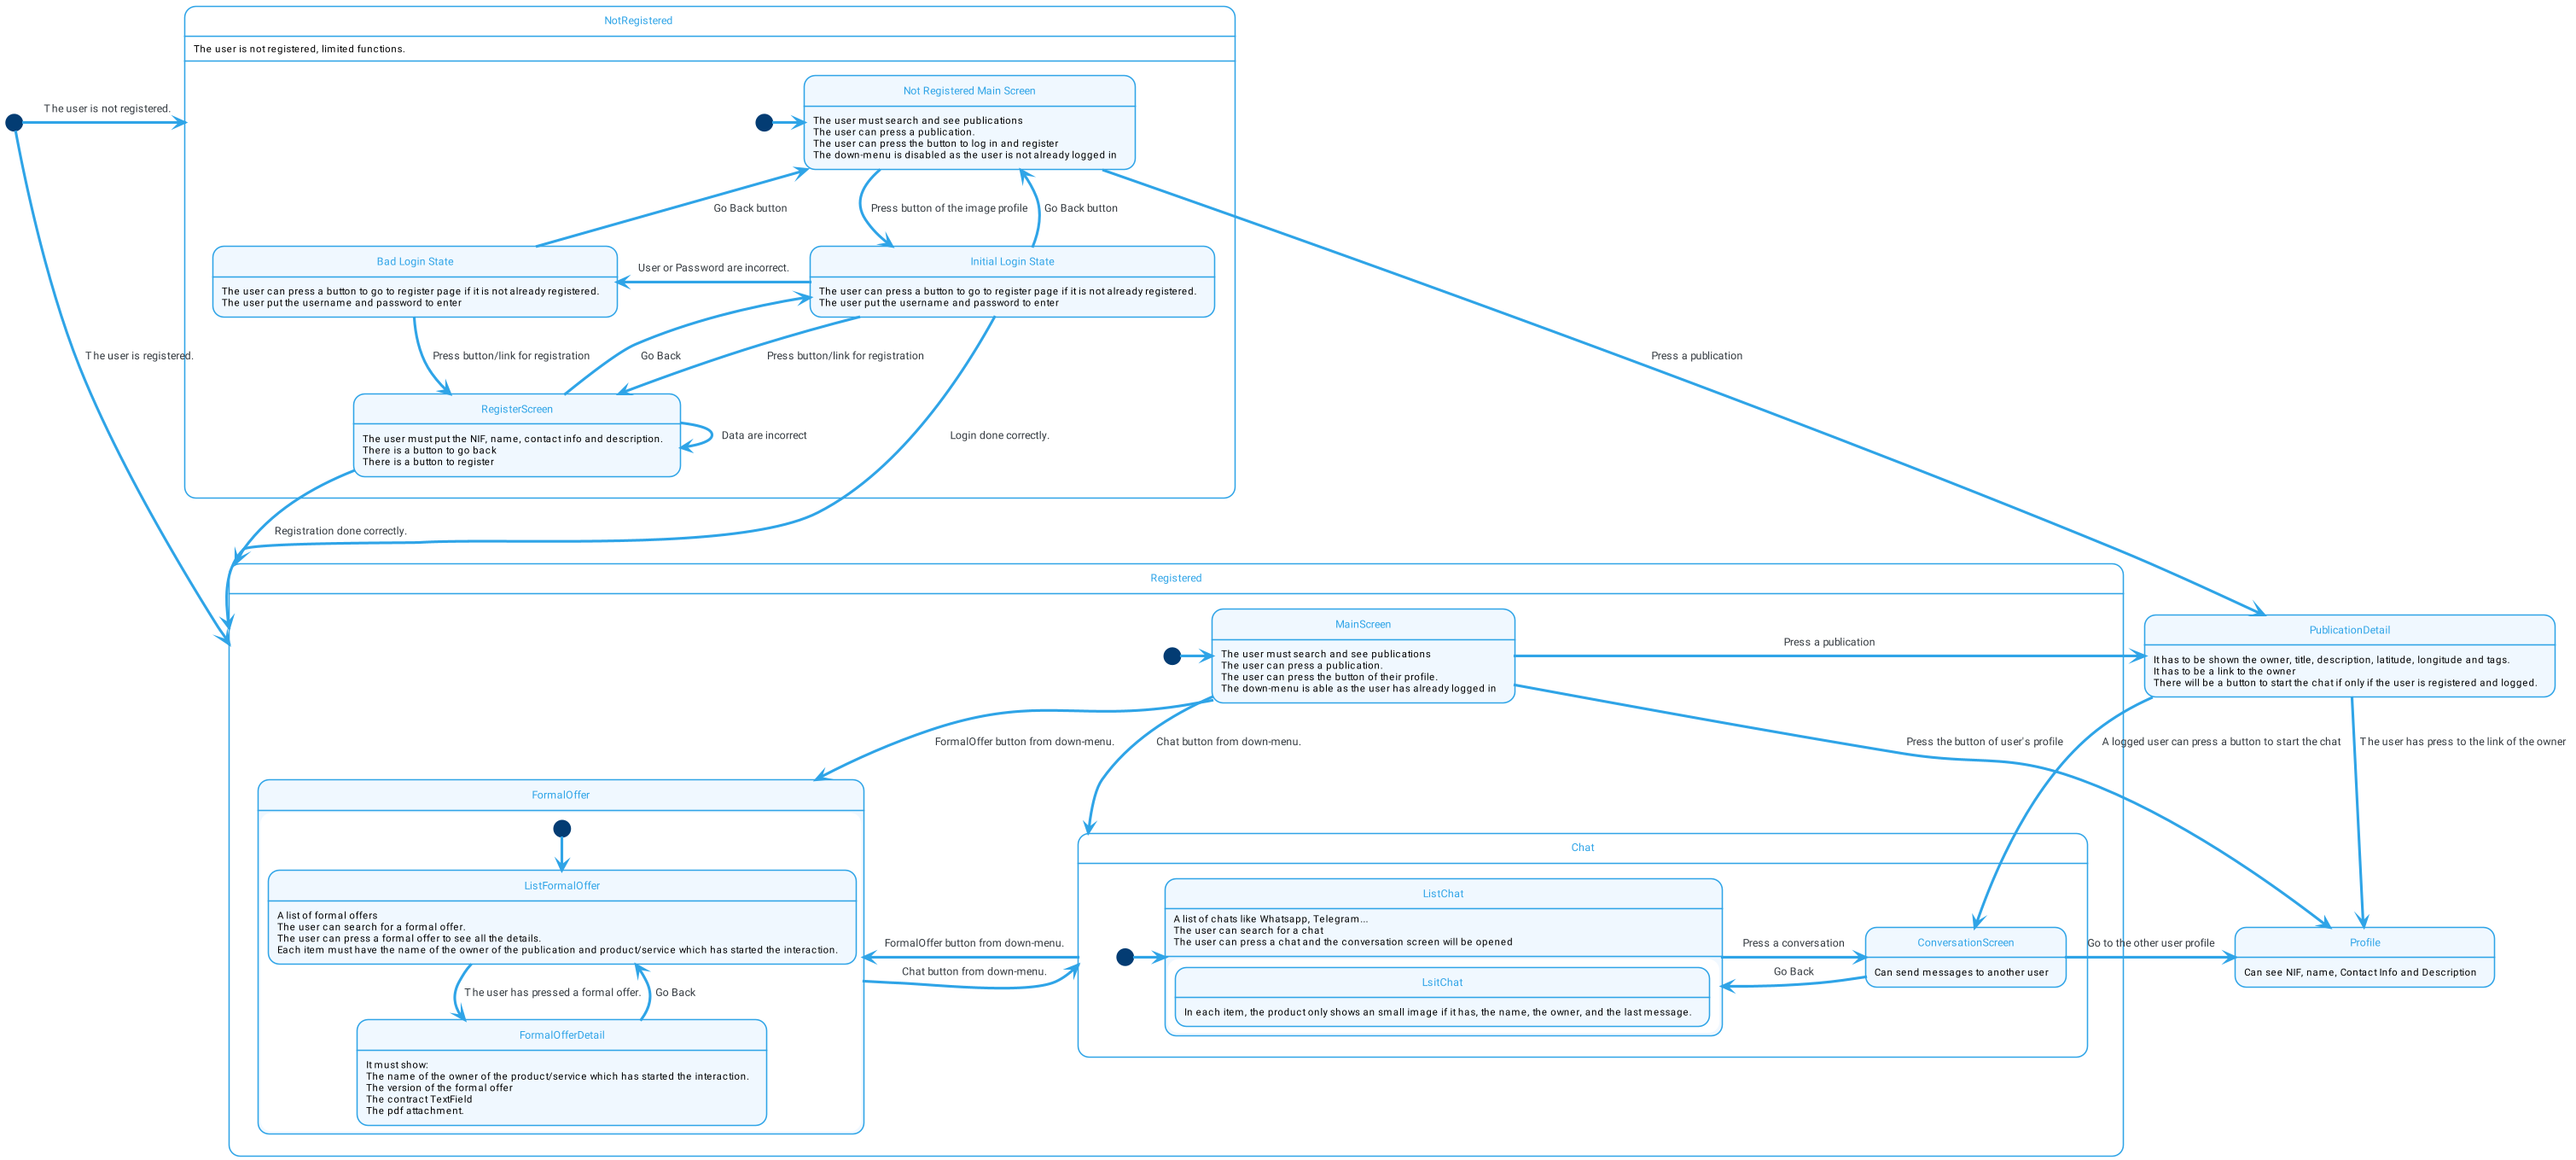
\includegraphics[width=14cm]{stateapp.png}
	\label{fig:stateapp}
	\caption{State diagram of the application.}
\end{figure}
\subsection{Mobile Application}
\subsubsection{Application}
% TODO change this.
In this section, you will encounter all the screens that the application has currently. The first three images correspond to the home, which lists some products, the list of chats, and the list of formal offers. This can be accessed when clicking at the bottom view. It can not be slides, as it was found confusing when using the images' carousel.\\
\\
The next page \ref{fig:mobile-screen-5} is the profile of an enterprise, which is triggered when clicking a logo of the enterprise, in the pages before. In the figure \ref{fig:mobile-screen-4}, the chat between two users can be seen. It also can be seen a formal offer version, and although a formal offer version can only be send by the owner of the product, it was though that showcasing both items in the mock would be better. The next image \ref{fig:mobile-screen-3} is the searcher of the app, that can be triggered when clicking the magnifying  glass icon. It has the history of the items searched, which can be deleted when clicking the trash button, or replicated when clicking the text.\\
\\
Finally, in the images \ref{fig:mobile-screen-2}, \ref{fig:mobile-screen-1}, it is shown the registration and the login screens.
\begin{figure}[H]
	\centering
	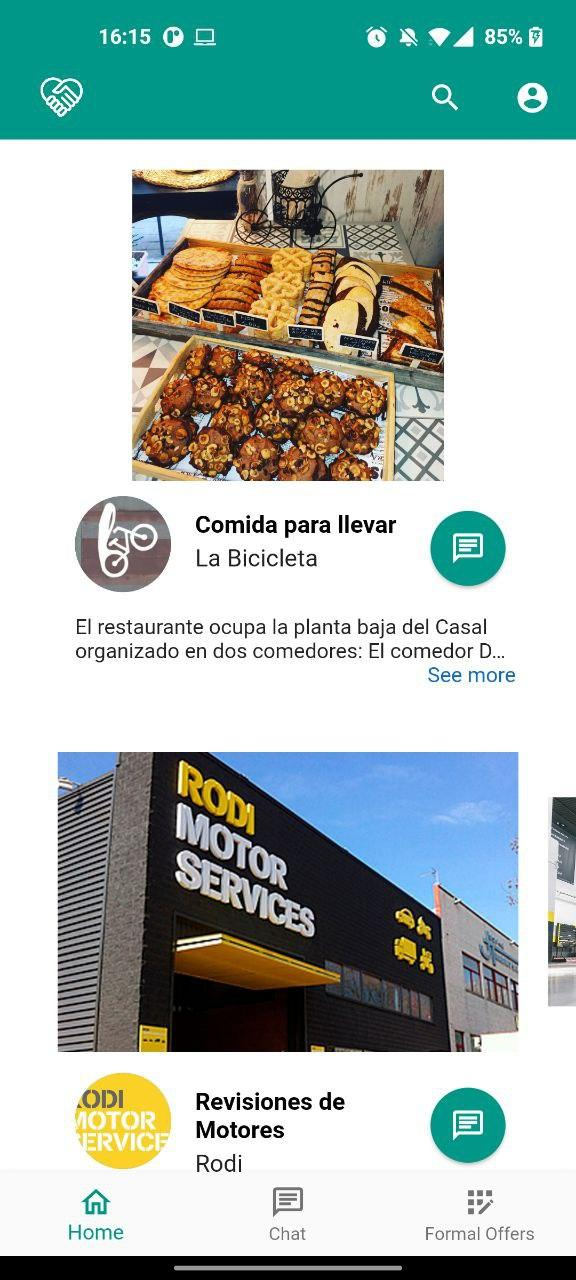
\includegraphics[width=0.5\linewidth]{img/mobile-screen-8.jpg}
	\caption{Home mobile screen, it lists the products}
	\label{fig:mobile-screen-8}
\end{figure}
\begin{figure}[H]
\centering
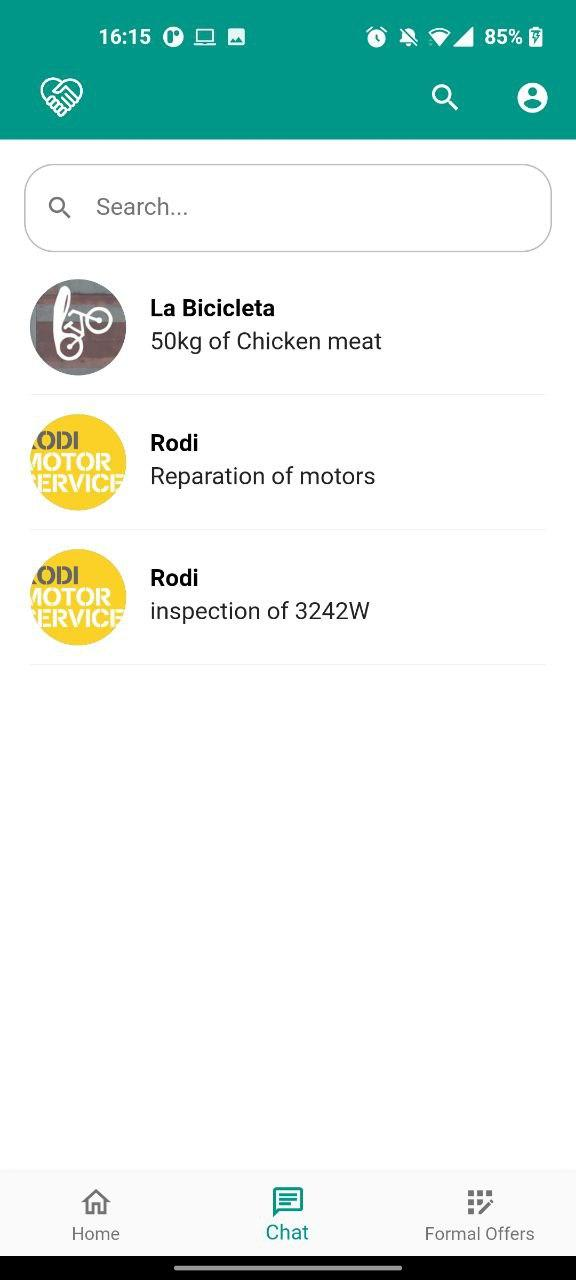
\includegraphics[width=0.5\linewidth]{img/mobile-screen-7.jpg}
\caption{List of the current chats.}
\label{fig:mobile-screen-7}
\end{figure}
\begin{figure}[H]
\centering
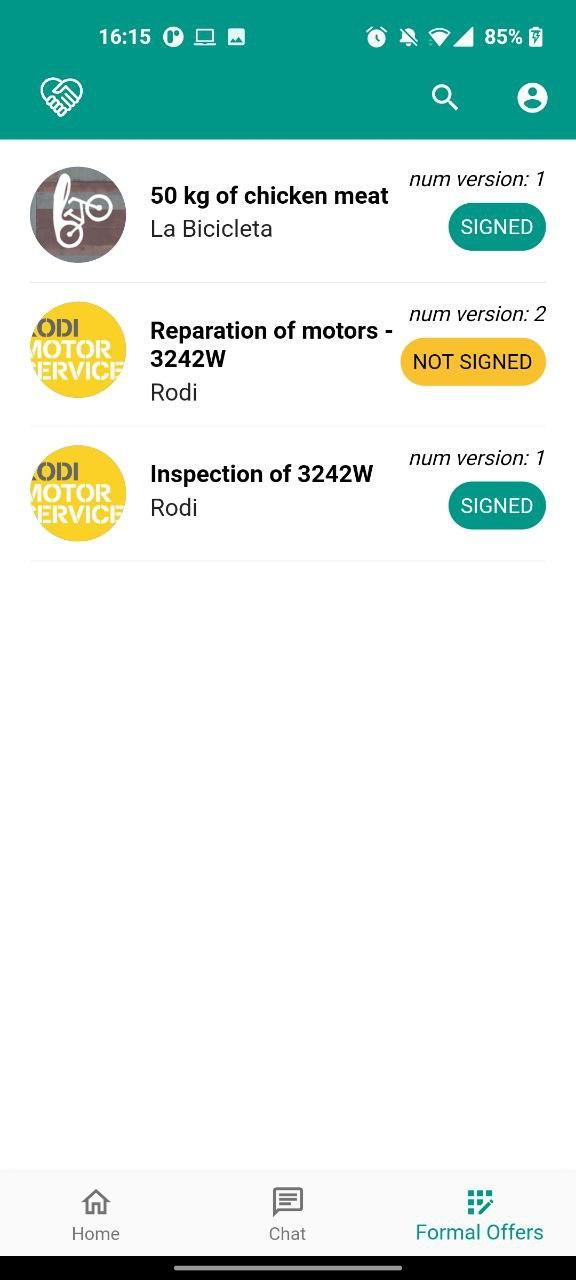
\includegraphics[width=0.5\linewidth]{img/mobile-screen-6.jpg}
\caption{List of the current formal offers.}
\label{fig:mobile-screen-6}
\end{figure}
\begin{figure}[H]
\centering

\includegraphics[width=0.5\linewidth]{img/mobile-screen-5.jpg}
\caption{Detail of an enterprise, it can be found when clicking the logo of it.}
\label{fig:mobile-screen-5}
\end{figure}
\begin{figure}[H]
\centering
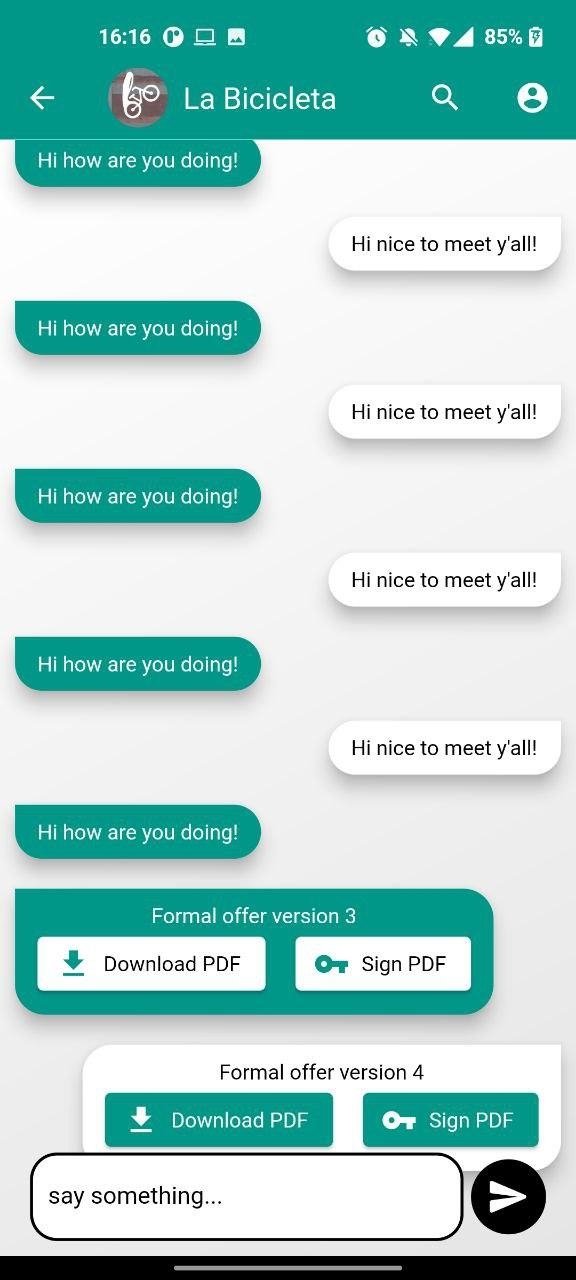
\includegraphics[width=0.5\linewidth]{img/mobile-screen-4.jpg}
\caption{Chat screen.}
\label{fig:mobile-screen-4}
\end{figure}
\begin{figure}[H]
\centering
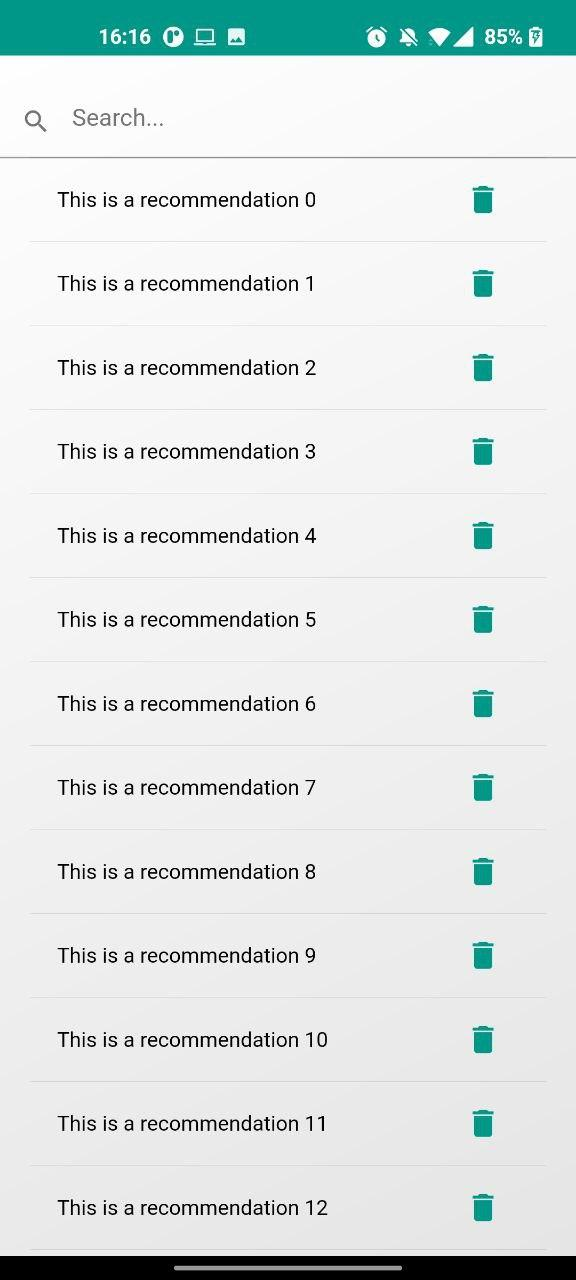
\includegraphics[width=0.5\linewidth]{img/mobile-screen-3.jpg}
\caption{Recommendations screen.}
\label{fig:mobile-screen-3}
\end{figure}
\begin{figure}[H]
\centering
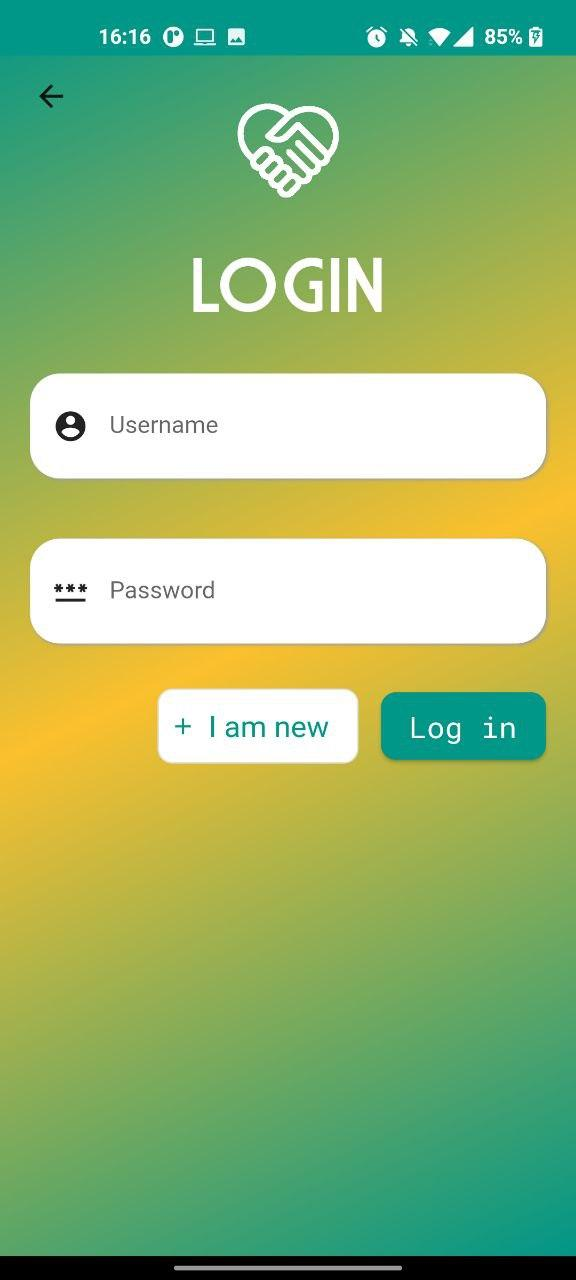
\includegraphics[width=0.5\linewidth]{img/mobile-screen-2.jpg}
\caption{Login view.}
\label{fig:mobile-screen-2}
\end{figure}
\begin{figure}[H]
\centering
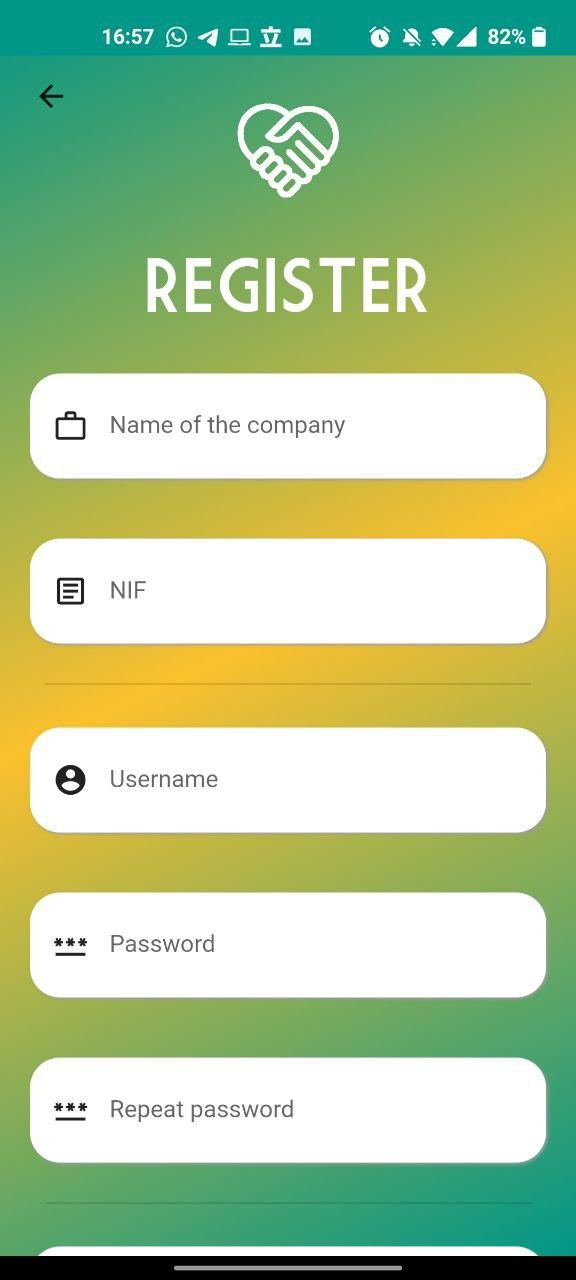
\includegraphics[width=0.5\linewidth]{img/mobile-screen-1.jpg}
\caption{Registration screen.}
\label{fig:mobile-screen-1}
\end{figure}


\subsection{Web Client}
\subsubsection{Application}
In this section it will be shown the changes that have graphically occurred in the views.
% left one as an example, as it wasn't needed that many items.
\begin{figure}[H]
  \centering
  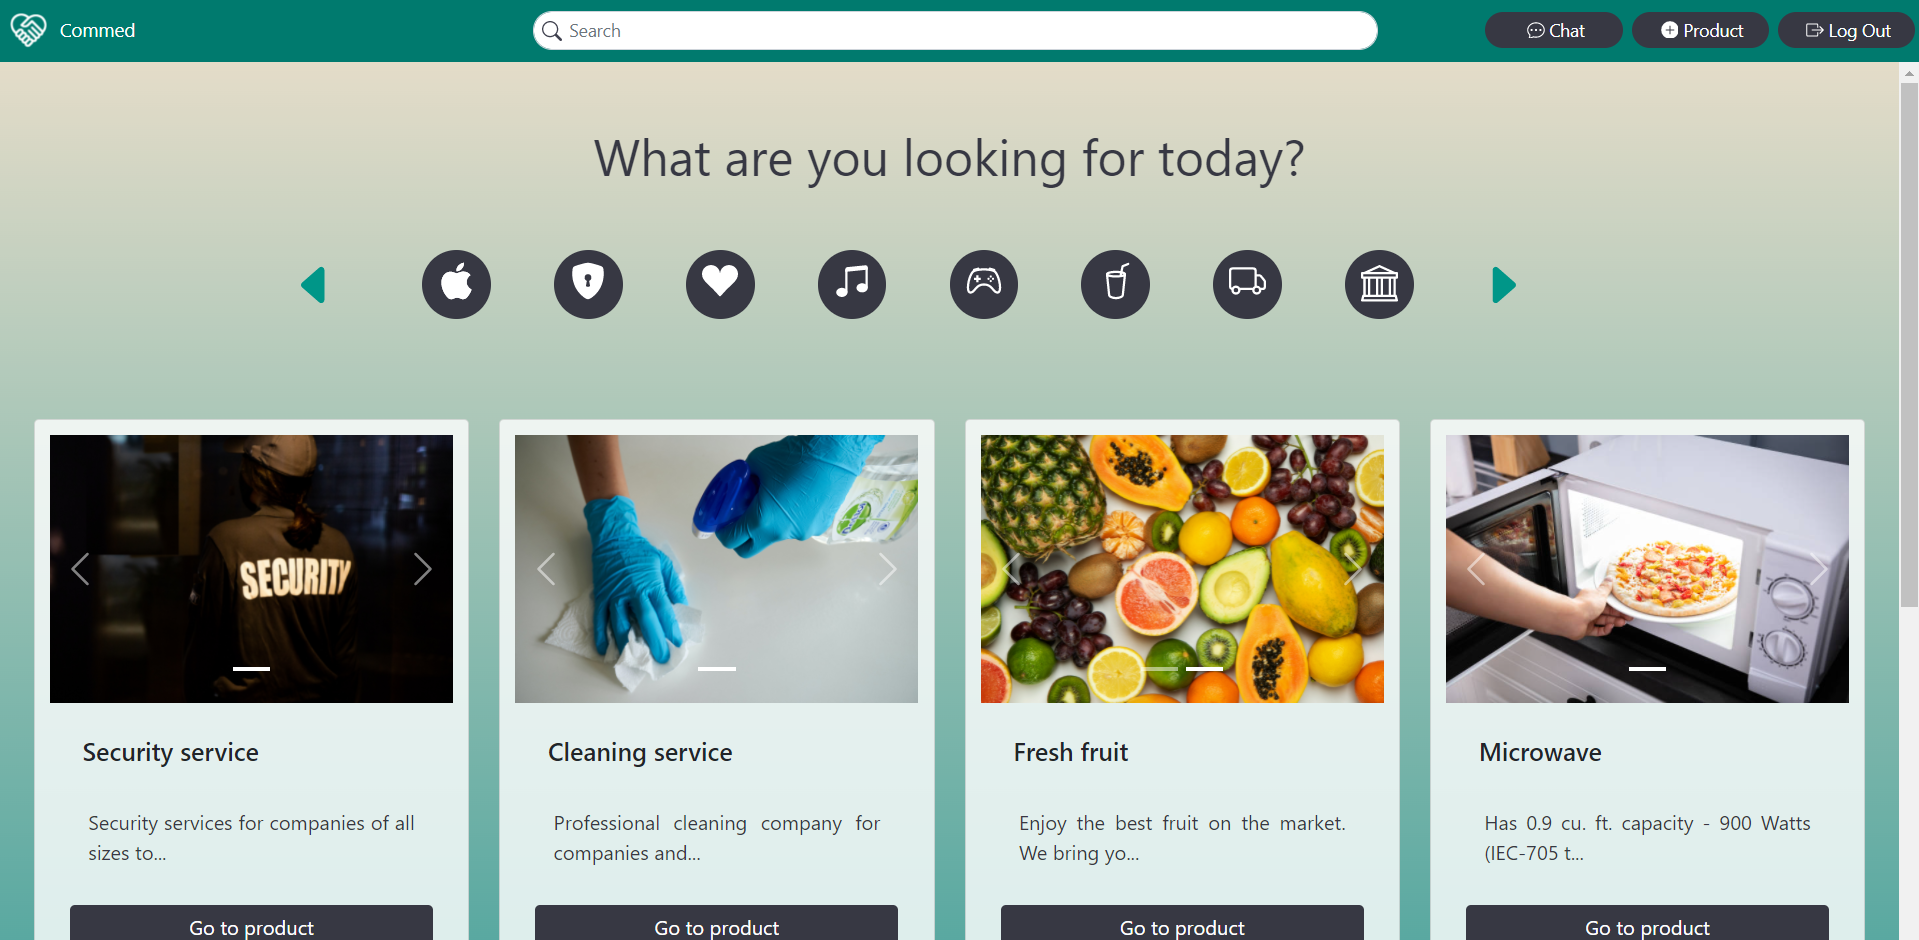
\includegraphics[width=0.5\linewidth]{img/webclient_2.png}
  \caption{Home screen.}
  \label{fig:webclient-screen-1}
\end{figure}

\section{Dailies}

\subsection{20-11-2021}
\begin{itemize}
	\item Creation of the items that shall be done by the end of the sprint
	\item Emina will work on polishing the app.
	\item Yassine will work on an accesibility and usability of the app.
	\item Quim will work on the product images CRUD, as it has a bug that needs to be fixed.
	\item Oriol will work on polishing the app, and connecting some endpoints in the app.
	\item Sergi will work in the implementation of the Chat in the backend.
\end{itemize}

\subsection{21-11-2021}
\begin{itemize}
	\item Everybody still worked on the same issues as the last time
\end{itemize}

\subsection{22-11-2021}
\begin{itemize}
\item Everybody worked on the same issues, and Oriol started focusing on integrating the application with the backend.
\end{itemize}

\subsection{29-11-2021}
\begin{itemize}
	\item Everybody worked on the same issues, but Emina finished her work.
\end{itemize}

\subsection{30-11-2021}
\begin{itemize}
	\item Emina and Sergi paired to solve some bugs on the chat application, as it didn't work
	on docker but it worked on local.
	\item All the other people were progressing on the same issues.
\end{itemize}

\subsection{1-12-2021}
\begin{itemize}
	\item Everybody worked on the same issues.
\end{itemize}


\subsection{10-12-2021}
\begin{itemize}
	\item The issues regarding the chat were discovered, so Sergi started working alone in fixing those issues.
	\item Emina started working on populating the database with more accurated users, to make the demonstrations better and the debugging of the application easier.
\end{itemize}

\subsection{11-12-2021}
\begin{itemize}
	\item Sergi finished the chat, and began implementing custom endpoints for listing all the chats and formal offers needed by the web application and the mobile application.
	\item Emina finished the database and started connecting the chat with the application.
	\item Quim aided Emina in the integration with the chat while he was stuck debugging the product images.
	\item Oriol integrated most of the app.
\end{itemize}

\subsection{12-12-2021}
\begin{itemize}
	\item Sergi changed some features for the chat, as they were requested to make the implementation easier for both clients.
	\item Emina debbuged the chat.
	\item Quim aided Emina in the integration with the chat, and made the product images CRUD work.
	\item Oriol integrated most of the app.
\end{itemize}

\subsection{13-12-2021}
\begin{itemize}
	\item Sergi aided Emina, Quim and Oriol, and also did the merges on two branches.
	\item Emina debbuged the chat and polished things
	\item Quim developed the images publishing on the frontend.
	\item Oriol integrated most of the app.
\end{itemize}

\subsection{14-12-2021}
\begin{itemize}
	\item Sergi aided some help and worked on the documentation.
	\item Emina finished the chat.
	\item Quim aided Emina.
	\item Oriol integrated the app completely.
\end{itemize}


\subsection{15-12-2021}
\begin{itemize}
	\item Sergi Quim and Oriol worked on the documentation
	\item Emina worked on the slides.
	\item Sergi hepled Nico put the financial case on the documentation.
\end{itemize}
\end{document}
